%%Target for future reference:
%http://www.journals.elsevier.com/environmental-modelling-and-software/

%Init document class
\documentclass[11pt]{article}

%Package for Authors on Title Page
\usepackage{authblk}

%Double Spacing Package
\usepackage{setspace}

%Biblatex Init
\usepackage[backend=bibtex, style=authoryear, citestyle=authoryear]{biblatex}
\bibliography{geoSIMEX}

%Figures Init
\usepackage{graphicx}
\graphicspath{ {images/} }

%Enable footnotes in tables
\usepackage{tablefootnote}

%Enable the \text{} command for use in equations
\usepackage{amsmath}

%Authors and Affiliations
\author[1]{Daniel Runfola}
\author[1]{Rob Marty}
\author[1]{Seth Goodman}
\author[1]{Michael LeFew}
\affil[1]{Institute for the Theory and Practice of International Relations, AidData, The College of William and Mary}
\renewcommand\Authands{ and }

%Title
\title{geoSIMEX: A Generalized Approach To Modeling Spatial Imprecision}

\usepackage{Sweave}
\begin{document}
\Sconcordance{concordance:master.tex:master.Rnw:%
1 21 1 1 5 2 1 1 0 9 1}
\Sconcordance{concordance:master.tex:./title.Rnw:ofs 35:%
1 11 1}
\Sconcordance{concordance:master.tex:master.Rnw:ofs 47:%
40 5 1}
\Sconcordance{concordance:master.tex:./abstract.Rnw:ofs 53:%
1 10 1}
\Sconcordance{concordance:master.tex:master.Rnw:ofs 64:%
47 2 1}
\Sconcordance{concordance:master.tex:./introduction.Rnw:ofs 67:%
1 58 1}
\Sconcordance{concordance:master.tex:master.Rnw:ofs 126:%
51 2 1}
\Sconcordance{concordance:master.tex:./dataMethods.Rnw:ofs 129:%
1 183 1}
\Sconcordance{concordance:master.tex:master.Rnw:ofs 313:%
55 2 1}
\Sconcordance{concordance:master.tex:./results.Rnw:ofs 316:%
1 20 1}
\Sconcordance{concordance:master.tex:master.Rnw:ofs 337:%
59 2 1}
\Sconcordance{concordance:master.tex:./discussion.Rnw:ofs 340:%
1 24 1}
\Sconcordance{concordance:master.tex:master.Rnw:ofs 365:%
63 2 1}
\Sconcordance{concordance:master.tex:./conclusion.Rnw:ofs 368:%
1 14 1}
\Sconcordance{concordance:master.tex:master.Rnw:ofs 383:%
67 2 1}
\Sconcordance{concordance:master.tex:./tables.Rnw:ofs 386:%
1 52 1}
\Sconcordance{concordance:master.tex:master.Rnw:ofs 439:%
71 2 1}
\Sconcordance{concordance:master.tex:./figures.Rnw:ofs 442:%
1 12 1 1 5 7 1}
\Sconcordance{concordance:master.tex:master.Rnw:ofs 463:%
75 2 1}
\Sconcordance{concordance:master.tex:./acknowledgements.Rnw:ofs 466:%
1 1 1}
\Sconcordance{concordance:master.tex:master.Rnw:ofs 468:%
79 5 1}


%-------------------------------------
%-------------------------------------
%Paper Sections 
%-------------------------------------
%-------------------------------------

%Title Page (title.Rnw)
\maketitle 
\begin{flushleft}
\textbf{Corresponding Author}:\\
Dr. Daniel Runfola\\
Institute for the Theory and Practice of International Relations, \emph{AidData}\\
427 Scotland Street, Williamsburg, VA 23185\\
Email: dsmillerrunfol@wm.edu
Telephone: 508.316.9109
Fax: 757.221.4650
\end{flushleft}


\newpage

%Toggle spacing for document
\doublespacing

%Abstract (abstract.Rnw)
\section{Abstract}
Spatial imprecision exists in nearly all spatial information - from census data to satellite information, the exact geographic location to which a measurement can be attributed is rarely known.
Following this, there is a large and growing set of literature examining how different classes of models can integrate information on spatial imprecision in order to more accurately reflect available data.
Here, we present a flexible approach - geoSIMEX - which can provide parameter and error estimates for both linear and non-linear models while adjusting for spatial imprecision.
Further, this approach can provide an estimate of the potential value of additional spatial information by distinguishing between traditional model error and additional errors introduced by imprecision.
We illustrate this approach through a case study leveraging a novel, publically available dataset recording the location of Chinese aid in Africa at varying levels of precision.
Using a difference-in-difference model, we integrate this information with satellite derived data on vegetation (NDVI) and a number of other spatially explicit covariates to examine if there is evidence Chinese aid has caused an increase or decrease in vegetation.
Following commonly employed procedures which do not incorporate spatial imprecision, we found that Chinese Aid had a negative impact on vegetation; once spatial imprecision was incorporated into our estimates through the geoSIMEX procedure no evidence of impact was found.
We use these findings to argue for the importance of incorporating spatial imprecision into analyses, and introduce new software in the R programming language to enable similar analyses for other purposes.

\textbf{Keywords}: SIMEX, Spatial Uncertainty, Spatial Data Integration, Simulation, Ecological Fallacy\\
\newpage

%Introduction
\section{Introduction}
The lack of exact geographic information on where measurements are obtained presents a barrier to research.
This has become increasingly evident as more scholars integrate geographic data from multiple sources - for example, census, satellite, and GPS sources - to try and establish causal or predictive relationships (c.f., EXAMPLES).
Many scholars have engaged in research seeking to integrate information on the precision of geographic data to improve the accuracy of modeling efforts, variably referred to as spatial (im)precision (CITE), spatial uncertainty (CITE), and spatial allocation (CITE).
This paper presents a generalizeable approach to integrating information on the precision of geographic data into both linear and non-linear models - geoSIMEX.
We illustrate the capability of geoSIMEX to provide more accurate parameter estimates than traditional approaches through a simulation framework. 
Using a novel dataset, we then apply both tradional models and a geoSIMEX model to examine the causal impact of Chinese Aid on vegetation in Africa.
We use this case study to illustrate the importance of including information on spatial imprecision into analyses.
Finally, we provide all data and an accompanying R package to users seeking to perform similar styles of analysis.

\subsection{Literature Review}
(dont include SIMEX here, just general lit on spatial uncertainty..  3 paragraphs.)


\subsection{(geo)SIMEX}
1 paragraph outlining the basic principles of SIMEX with cites..

1 paragraph showing cases where SIMEX has been used with cites.

\par
In geoSIMEX, we take this approach and modify $\lambda$ to capture the degree of spatial imprecision in a given dataset, relative to the maximum amount of imprecision that could be observed.
The practical need for a geographic version of SIMEX can be demonstrated through a hypothetical example, in which a researcher seeks to measure the degree to which the amount of precipitation across 200 fields can explain the number of apples grown in each field.
These hypothetical researchers measure precipitation in each of 200 fields using satellite imagery, and counts each of the apples by hand.
In the simplest form, these researchers then use these measurements to model the relationship between rainfall and apples following:
\begin{equation}\label{eq:precip}
\text{CountOfApples} = \beta_{0} + \theta * \text{Rainfall} + \sum{\beta_{j} * X_{j}} + \epsilon
\end{equation}
\noindent in which $\beta_{j}$ and $X_{j}$ represent vectors of parameter estimates and controls, respectively. 
In this equation, a common goal would be to estimate $\theta$ with a high degree of accuracy, as this parameter helps to explain the degree to which precipitation impacted the count of apples.
\par
In this example, if each field was a perfect square of the same resolution as the satellite imagery (and had perfect overlap), then the measurements of rainfall would have no measurement error due to imprecision.
In practice, this rarely is the case, and thus the parameter $\theta$ can be biased due to imprecision in measurements.
Consider, for example, the worst case of imprecision in which a coarse reolution satellite sensor provides only one measurement of rainfall for every crop.
A responsible researcher seeking to use this data might leverage a model averaging framework to overcome concerns of the ecological fallacy - i.e., randomly distributing rainfall to each crop, fitting equation \ref{eq:precip}, and repeating this hundreds of times to estimate the range of possible coefficients that could be observed given the available data.
However, in cases of complete spatial imprecision, these estimates will be heavily biased towards 0.
This has two implications - first, the mean estimated coefficient will likely under-estimate the true coefficient, and second the distribution of possible coefficients (i.e., at a 95\% confidence level) will be centered at this biased coefficient.  
This suggests that not only can mean estimates be incorrect, but under cases of spatial imprecision statements regarding the significance of variables can also be biased.
\par
While it is rare that satellite measurements perfectly line up with units of analysis, it is also rare that researchers only have one measurement for all units of analysis.
More reasonably, researchers commonly have a mixture - i.e., satellite imagery that may cover portions of some crops but not others, leading to variable imprecision across the study area.
geoSIMEX takes advantage of the known level of precision in the data available ot the research (which we define as $\lambda$), and intentionally adds imprecision to establish the relationship between additional imprecision and coefficient bias.
The geoSIMEX procedure then uses this relationship to back-extrapolate to an unbiased coefficient estimate, i.e. the value at $\lambda$ = 0.
Finally, we employ a bootstrapping procedure to estimate the additional variance attributable to spatial imprecision.





\newpage

%Data and Methods
\section{Data and Methods}
This study leverages a novel dataset on the location of Chinese international aid in Africa available at varying levels of precision (i.e., the exact location of each aid project is not always known).  
It integrates this information with a variety of other ancillary datasets, including the NASA Long Term Data Record (LTDR) to examine the causal impact of Chinese aid on vegetation.  
Employing geoSIMEX, we use this case study to illustrate the importance of incorporating information on spatial imprecision into analyses.
\subsection{Data}
To conduct this analysis, a new dataset on the location of Chinese aid is derived through a methodology designed to Track Underreported Financial Flows (the TUFF methodology).  
This dataset is merged with a number of existing datasets, retrieved from publically available sources as described below.
\subsubsection{Study Area and Scope}
(Placeholder for study scope)
\subsubsection{Tracking Underreported Financial Flows (TUFF)}
Unlike many donors, China does not publically report the international aid they send (CITE).
(Placeholder for TUFF details)
Due to the considerable spatial imprecision generated by the TUFF process, we use this variable as an illustrative case of how the geoSIMEX procedure can be used to provide better estimates than traditional approaches.
\subsubsection{Ancillary Datasets}
Covariate data is collected from a variety of sources, summarized in table \ref{data_source_table}.
Our outcome measure - fluctuation in NDVI - is derived from the NASA Long Term Data Record (LTDR) dataset.
While relatively coarse resolution, this dataset represents the longest consistent record of NDVI available at the global scale.
To facilitate our difference-in-difference modeling efforts, we further select a number of covariates we believe could also impact shifts in NDVI (other than Chinese aid).
These include:
\begin{enumerate}
\item{Long-term climate data from the University of Delaware, providing precipitation and temperature data at a monthly time-step for the full data record, which is permuted to produce yearly mean, minimum, and maximum values for each project location.}
\item{Population Data is retrieved from CIESIN at Columbia University, specifically leveraging the Gridded Population of the World (GPW) data record.}
\item{Slope and Elevation data are derived from the Shuttle Radar Topography Mission (SRTM).}
\item{Distance to rivers is calculated based on the USGS Hydrosheds database.}
\item{Distance to roads is calculated based on the Global Roads Open Access Dataset (gRoads), which represents roads circa 2010, though the actual date of datasets is highly variable by country.}
\item{Urban travel time, calculated by the European Commission Joint Research Centre.}
\item{Nighttime Lights are retrieved from the NOAA Earth Observation Group, calculated from the Department of Defense Defense Meteorological Satellite Program (DMSP).  Lights values are temporally intercalibrated following the procedure outlined in \cite{weng_global_2014}}
\end{enumerate}
Each of these datasets are processed and aggregated according to their average values within each district included in this analysis.  
Further, the size of districts are controlled for to mitigate the challenge of variably-sized districts across the study area.
In cases where covariates were measured at a resolution coarser than the unit of observation, the relative area of overlap was used to generate a weighted mean; the geoSIMEX procedure described below can be leveraged to account for such spatial imprecision, but is omitted from this analysis.
Further information on this decision can be found in the discussion.

\subsection{Methods}
Two different modeling processes are followed.  First, we use a monte carlo simulation procedure to illustrate the relative accuracy of geoSIMEX as contrasted to other procedures.  Second, we apply geoSIMEX to the case of Chinese Aid in Africa.

\subsubsection{geoSIMEX}
We employ geoSIMEX to identify the impact of Chinese Aid on vegetation, measured by a satellite-derived measure of NDVI.
We specifically seek to adjust for bias in the relative spatial imprecision of where Chinese Aid is located - imprecision largely due to the lack of formal information published by the Chinese government.
We describe this process through an illustrative example, in which we attempt to solve the following simplified equation:
\begin{equation}
NDVI = \theta * \text{Chinese aid} + \epsilon
\label{eqn:ndvi_aid}
\end{equation}
where, for the sake of example, Chinese aid is defined to be causally and positively related to a measure of NDVI by a one-to-one relation (e.g., $\theta$ = 1), and $\epsilon$ is a random error term. 
Aid is measured with spatial imprecision, and through using geoSIMEX we account for the spatial uncertainty to accurately estimate the model coefficient, $\theta$. 
\par
In figure \ref{fig:nepal_ex}, we present a hypothetical country with sixteen districts for which we seek to solve equation \ref{eqn:ndvi_aid}. 
Four of these sixteen units of analysis, districts 5,6,7, and 8 are distinguished on the map. 
Within this study area, a hypothetical data set contains three geocoded Chinese aid project locations of various levels of spatial precision, projects A, B, and C. 
Project A is assigned a coordinate pair in District 5 and had strong documentation, resulting
in precise geographic information (i.e. an exact latitude and longitude). 
Due to weaker project documentation, location B has a precision level indicating that it was allocated anywhere in the region that includes districts 5,6,7, and 8. 
Project C has very uncertain spatial information, such that it may be anywhere in the country. 
The area (in square kilometers) of the unit of analysis in which each project location may have been allocated gives us the size of the project location’s area of coverage, which is summarized in table \ref{precision_example}.
Using the spatial overlap between each region of interest (the sixteen districts) and the area an international aid project might exist in, we calculate a probability that each district contains a given project:

\begin{equation}\label{eq:overlaps}
V_{t} = \sum_{S}^{s=1}U_{s}\left ( \frac{a_{st}}{\sum_{T}^{t=1}a_{st}} \right )
\end{equation}

\noindent This represents the "no information" case - i.e., probabilities are only based on geographic overlap, as opposed to integrating other factors which might mediate where aid is allocated.
This equation can be modified to incorporate more information on spatial location, thus allowing a researcher to trade off additional assumptions or information about factors that mediate spatial allocation in exchange for higher degrees of spatial precision (i.e., through dasymetric mapping approaches).
\par
We use these probabilities in a modified version of the SIMEX procedure, geoSIMEX.  
In traditional SIMEX, measurement error is captured through scaling an estimated distribution of errors.
In our context, greater spatial imprecision is reflected by increasing the area of coverage of a project, thus expanding the probability a project could be located in a wider set of units of analysis. 
geoSIMEX exploits the fact that greater spatial imprecision will bias results towards 0 - i.e., if all data was measured at the country scale and every district had an equal probability of receiving aid, any results found using districts as the unit of analysis would be the equivalent of random noise.
geoSIMEX (a) calculated the initial level of spatial imprecision in a given dataset, and then (b) simulates additional spatial imprecision to establish this relationship between spatial imprecision and covariate bias. 
Based on this relationship, it extrapolates to a point with zero spatial imprecision, thus providing an estimate of the unbiased coefficient.
\par

\textbf{The first step} of geoSIMEX is to calculate the initial level of spatial imprecision in the given dataset, defined by $\lambda$.
To reflect imprecision across a given set of international aid projects and a set of units of analysis (i.e., districts), we calculate (\begin{math}\lambda\end{math}) following:

\begin{equation}\label{lambda}
\lambda = \frac{\sum_{i}^{P}Area \ of \ Coverage_i}{\sum_{i}^{P}Total \ Possible \ Area \ of \ Coverage_i}
\end{equation}

\noindent where $i$ is an individual project out of $P$ total Chinese Aid projects. $Area \ of \ Coverage_i$ is project $i$'s known area of coverage defined by the available documentation - i.e., the geographic area across which a project could be located. 
$Total \ Possible \ Area \ of \ Coverage_i$ is the area of coverage of project $i$ under complete spatial imprecision - e.g., the geographic area of the study area.
\par
If the latitude and longitude of every aid project was known, $\lambda$ would resolve to 0---indicating zero spatial imprecision. 
If spatial data was only available for the entire study area (e.g., aid provided for general budget support without indication of where the project was allocated), $\lambda$ would resolve to 1---indicating 100\% spatial uncertainty. 
In practice, combinations of different levels of precision result in $lambda$ values between these two extremes, providing a single linear measurement of spatial imprecision.
\par
\textbf{The second step} involves estimating a naive model (which can be of variable functional forms; for illustration we use ordinary least squares regression), where imprecision in aid is ignored. 
For each unit of observation, the value of aid used for modeling is the expected value of aid calculated following the geographic overlap-based probabilities described in (EQUATION!!).
In figure \ref{fig:steps}, we provide an example of the geoSIMEX procedure is applied to a dataset with an initial $\lambda$ value of 0.4, indicating the set of data provided was of moderate spatial precision relative to the units of observation.
In this figure, the x-axis represents the $\lambda$ value (spatial imprecision) for a dataset, with higher values indicating more imprecision.
The y-axis represents the estimated value of $\theta$ in equation \ref{wealth_aid}.
In \ref{fig:steps}a, the orange line represents the 95\% confidence interval of the coefficient on aid in this naive model. 
The horizontal black line represents the true model coefficient ($\theta$ = 1), which the naive model fails to capture.
\par 
In \textbf{the third step}, additional imprecision is simulated by randomly decreasing the precision of observations (in this case, Chinese Aid projects). 
For example, a project that has a measurement with an exact latitude and longitude will randomly be assigned a lower level of precision - i.e., a county, state, or even the entire country. 
Using these new, reduced levels of precision a model is fit in an identical fashion to step 1, and the estimated $\theta$ parameter, standard errors of the model,ad $\lambda$ value for a given permutation are saved.
This process is repeated 10000 times. 
In figure \ref{fig:steps}b, the black points represent individual iterations, with the saved model coefficients (y axis) and their associated $\lambda$ (x axis) values. 
\par
\textbf{The fourth step} subdivides this set of iterations into three equally-sized bins based on the level of spatial uncertainty ($\lambda$) of the aid variable (e.g., if $\lambda$ values range from 0.4 to 1, coefficients are separated into bins of 0.4-0.6, 0.6-0.8, and 0.8-1). 
Average coefficient and $\lambda$ values are calculated within each bin, represented as red dots in figure \ref{fig:steps}c. 
A quadratic trend is fit on the resulting average coefficient and lambda values. 
The trend is then extrapolated back to $\lambda=0$, thus providing an estimate of $\theta$ with perfect spatial precision. 
In figure \ref{fig:steps}d, the red line represents the extrapolated trend, and the blue dot represents the extrapolated estimate of the coefficient on aid. 
\par 

\textbf{In the fifth step}, the variance and standard errors of these estimates are calculated. 
We employ a bootstrapping method to calculate the component of the standard error resulting from spatial imprecision. Here, a point from each bin is sampled, a quadratic trend is fit on the resulting values, and the trend is extrapolated back to $\lambda$ = 0. 
This process is repeated 10000 times (defined as $R$). 
In figure \ref{fig:steps}e, each blue line represents one extrapolated trend and $\lambda$ = 0 estimate. 
We use a variance equation originally developed to capture model selection uncertainty to seperately incorporate both original standard errors and the additional error from spatial imprecision (CITE Burnham and Anderson):

\begin{equation}\label{variance}
var(\hat{\bar{\beta}}) = \sum_i^R \frac{1}{R} \{ var(\hat{\beta_i}) + (\hat{\beta_i}-\hat{\bar{\beta_i}})^2 \}
\end{equation}

\noindent where $R$ is the number of extrapolated coefficients (in this example, 1000). 
$var(\hat{\beta_i})$ is the standard error of each extrapolated coefficient, calculated by fitting a quadratic trend on the standard error estimates from each bin extrapolating back to $\lambda=0$ and collecting the resulting standard error value. 
$(\hat{\beta_i}-\hat{\bar{\beta_i}})^2$ captures the component of the variance from spatial uncertainty, where each extrapolated coefficient estimate is subtracted by the mean of all extrapolated coefficient estimates.  

\subsubsection{Simulations}


\subsubsection{Chinese Aid in Africa}
\newpage

%Results
\section{Results}
Placeholder
\newpage

%Discussion
\section{Discussion}
Placeholder
\newpage

%Conclusion
\section{Conclusion}
Placeholder
\newpage

%Tables
\section{Tables}
%Table 1
\begin{table}[!htbp]
\begin{tabular}[h]{|p{4.5cm}||p{7cm}|}
\hline
\multicolumn{2}{|c|}{\texttt{Data Sources}} \\
\hline
\textbf{Data Name} & \textbf{Source} \\
\hline
Chinese Aid Locations & AidData\begin{math}\tablefootnote{http://china.aiddata.org}\end{math} \\
\hline
Gridded Population of the World & Center for International Earth Science Information Network\tablefootnote{http://sedac.ciesin.columbia.edu/data/collection/gpw-v3/sets/browse} \\
\hline
Nighttime Lights & Defense Meteorological Satellite Program\tablefootnote{Stable Lights retrieved from http://ngdc.noaa.gov/eog/dmsp.html}\\
\hline
Precipitation and Temperature & University of Delaware (\cite{willmott_terrestrial_2001})\tablefootnote{Variables derived from these product included the average precipitation (P) and temperature (T) before a project was implemented (from 1992), the linear trend in P and T from 1992 to the project implementation, the average temperature from the date the project was implemented until the end of the temporal record(2012), and the post-project trend through 2012. Absolute measurements of each variable were also retained. } \\
\hline
Urban Travel Time & European Commission Joint Research Centre\tablefootnote{http://forobs.jrc.ec.europa.eu/products/gam/download.php}\\
\hline
Distance to Rivers & World Wildlife Fund \tablefootnote{http://hydrosheds.cr.usgs.gov/index.php}\\
\hline
Vegetation & NASA LTDR\tablefootnote{http://ltdr.nascom.nasa.gov/cgi-bin/ltdr/ltdrPage.cgi} \\
\hline
Distance to Roads & CIESIN gRoads\tablefootnote{http://sedac.ciesin.columbia.edu/data/set/groads-global-roads-open-access-v1} \\
\hline
\end{tabular}
\caption{Data sources used in this analysis.}\label{data_source_table}
\end{table}

\newpage
%Table 2 - Precision  Example
\begin{table}[!htbp]
	\begin{tabular}{| l | l | l |}
	\hline
	Project Location & Relative Precision & Known Aid Location (Geographic Size)\\
    \hline
    A &  Very High & Populated Area in District 5 (3 $\text{km}^2$) \\ \hline
    B &  Moderate & Districts 5-8 (32,000 $\text{km}^2$) \\ \hline
    C &  Very Low & Entire Country (112,500 $\text{km}^2$) \\ \hline
	\end{tabular}
	\caption{Example of the geographic area across which aid projects might be located given limited spatial information.}\label{precision_example}
\end{table}
\newpage

%Figures
\section{Figures}

\begin{figure}[!htbp]
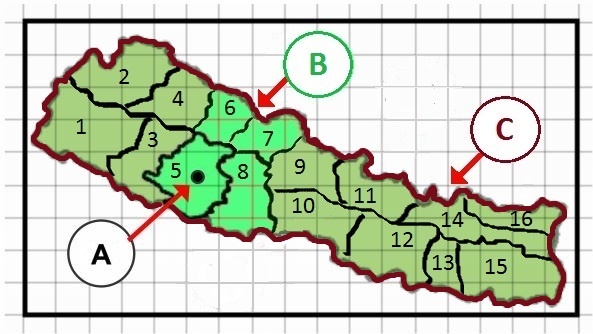
\includegraphics{nepal_ex}
\caption{Hypothetical example of spatial imprecision in aid allocation.}\label{fig:nepalex}
\end{figure}

\begin{figure}[!htbp]
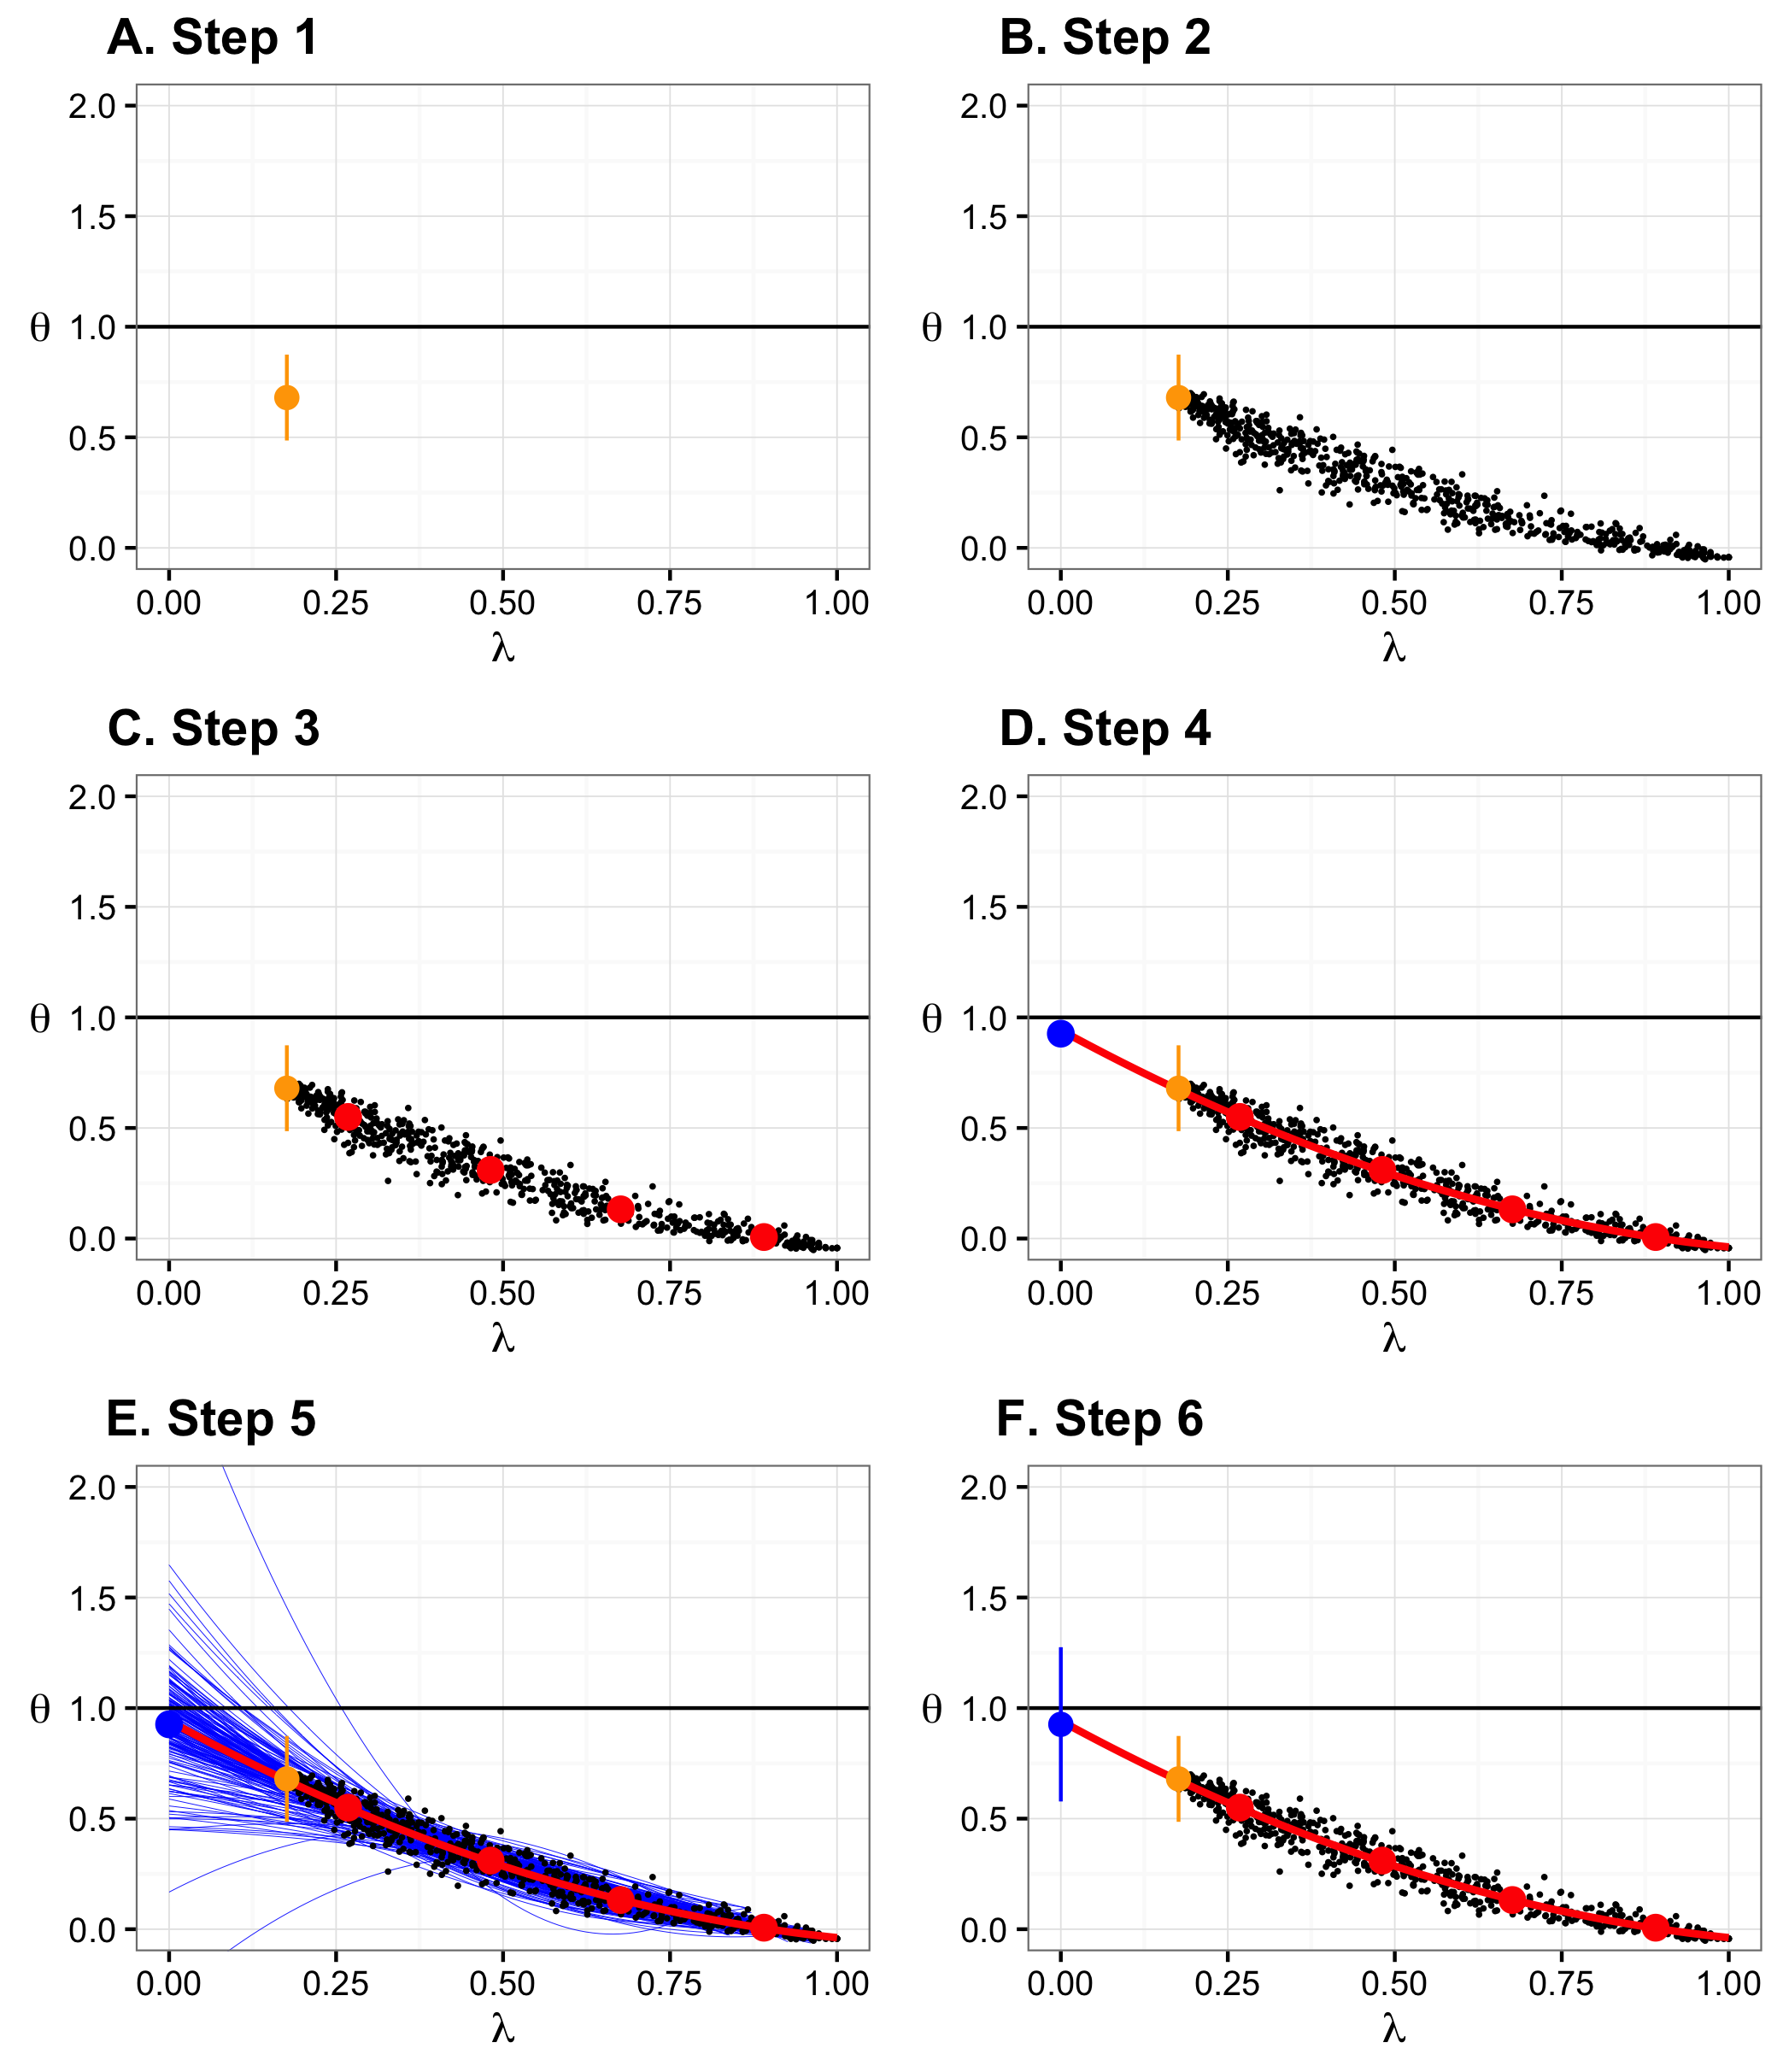
\includegraphics{steps}
\caption{Steps of the geoSIMEX procedure.}\label{fig:steps}
\end{figure}
\newpage

%Acknowledgements
\section{Acknowledgements}
Remember: USAID grant, Relevant SciClone grants, Ben Dykstra, Ariel
\newpage

%Bibliography
\printbibliography

\end{document}
